\documentclass{article}
\usepackage{listings}
\usepackage{graphics}
\usepackage{graphicx}
\usepackage{hyperref}
\usepackage{amssymb}
\usepackage{float}
\usepackage{amsmath}
\usepackage{longtable}
\usepackage{xcolor}

\definecolor{codegreen}{rgb}{0,0.6,0}
\definecolor{codegray}{rgb}{0.5,0.5,0.5}
\definecolor{codepurple}{rgb}{0.58,0,0.82}
\definecolor{backcolour}{rgb}{0.95,0.95,0.92}

\lstdefinestyle{mystyle}{
    backgroundcolor=\color{backcolour},   
    commentstyle=\color{codegreen},
    keywordstyle=\color{magenta},
    numberstyle=\tiny\color{codegray},
    stringstyle=\color{codepurple},
    basicstyle=\ttfamily\footnotesize,
    breakatwhitespace=false,         
    breaklines=true,                 
    captionpos=b,                    
    keepspaces=true,                 
    numbers=left,                    
    numbersep=5pt,                  
    showspaces=false,                
    showstringspaces=false,
    showtabs=false,                  
    tabsize=2
}

\lstset{style=mystyle}


\title{Chapter 1 \\
Mengenal Kecerdasan Buatan dan
Scikit-Learn}
\author{Rizal Ramadhan (1184033)}
\date{March 2021}

\begin{document}

\maketitle 
\section{Teori}
Kecerdasan Buatan atau biasa disebut Artificial Intelligence (AI) adalah teknologi yang dibuat oleh manusia yang dimodelkan dalam bentuk mesin dan diprogram agar bisa berpikir seperti halnya manusia, yang bisa melakukan pekerjaan-pekerjaan yang umumnya memerlukan tenaga manusia atau kecerdasan manusia. 

Sama halnya seperti manusia, AI juga membutuhkan pengalaman dan data untuk dijadikan pengetahuan supaya kecerdasannya bisa lebih baik lagi. Proses belajarnya berjalan dengan sendirinya berdasarkan pengalamannya saat digunakan oleh manusia. Point penting dalam proses AI yaitu learning, reasoning, and self correcting.

\subsection{Sejarah}
"Intelligence" berasal dari bahasa Latin yaitu "intelligo" yang berarti "saya paham". Arti dasar dari intelligence ialah kemampuan untuk memahami dan melakukan aksi.

Sejarah kecerdasan buatan dimulai pada zaman kuno namun sebagai mitos, cerita dan desas-desus tentang makshluk buatan yang diberkahi oleh pengrajin. Karya ini memuncak saat penemuan komputer digital yang diprogram pada tahun 1940-an.
Istilah kecerdasan buatan pertama kali dikemukakan pada tahun 1956 di Konferensi Darthmouth. Sejak saat itulah ia terus dikembangkan sampai saat ini.

Pada akhir 1955, Newell dan Simon mengembangkan  The Logic Theorist, program AI pertama. Program ini berdampak besar dan menjadi batu loncatan penting dalam mengembangkan bidang AI. Pada tahun 1956 John McCarthy dari  Massacuhetts Institute of Technology dianggap sebagai bapak AI, menyelenggarakan konferensi untuk menarik para ahli komputer bertemu, dengan  nama kegiatan “The Dartmouth summer research project on artificial intelligence.”   Konferensi Dartmouth itu mempertemukan para pendiri dalam AI, dan bertugas untuk meletakkan dasar bagi masa depan  pemgembangan dan penelitian AI. Pada  tahun 1960 hingga 1970, muncul berbagai dikusi bagaimana komputer dapat meniru sedetail mungkin pada kemampuan otak manusia, dimana saat itu dapat dikategorikan sebagai “classical AI”. Pada tahun 1980, computer semakin mudah diperoleh dengan harga yang lebih murah, lalu menjadikan berbagai riset di bidang kecerdasan buatan semakin berkembang pesat pada berbagai universitas.

\subsection{Perkembangan Kecerdasan Buatan}
\begin{itemize}
\item{Awal Perkembangan AI ( 1952 - 1969 )}
Diawali dengan kesuksesan Newell dan Simon dengan sebuah program yaitu General Problem Solver yang dirancang untuk memuai penyelesaian masalah secara manusiawi, kecerdasan buatan mengalami banyak kesuksesan.

1959 Nathaniel Rochester dari IBM dan mahasiswa-mahasiswanya juga mengeluarkan program kecerdasan buatan dengan nama Geometry Theorm Prover yang dapat mengeluarkan suatu teorema menggunakan aksioma-aksioma yang ada.

1963 James Slagel juga membuat program yang mampu menyelesaikan masalah integral tertutup untuk matakuliah kalkulus.

Selanjutnya pada 1986 Tom Evan juga membuat program analogi yang dapat menyelesaikan masalah analogi geometris yang ada pada tes IQ.

\item{Perkembangan kecerdasan buatan Melambat ( 1966 - 1974 )}
Pada Tahun 1966 hingga 1974 perkembangan kecerdasan buatan mulai melambat, hal ini disebabkan oleh 3 kesulitan utama yaitu:

Pertama, program-program yang bermunculan hanya mengandung sedikit pengetahuan pada subjeknya. Program tersebut berhasil hanya karena manipulasi sederhananya saja.

Kedua, banyaknya masalah yang harus diselesaikan oleh kecerdasan buatan tersebut.

Ketika, Terdapat beberapa batasan pada struktur dasar yang digukanakan untuk menghasilkan perilaku intelligensia.

\item{Sistem Berbasis Pengetahuan ( 1969 - 1979 )}
Pada tahun 1969-1979 Ed Feingenbaum, Bruce Buchanan dan Joshua Lederberg membuat program untuk memecahkan masalah struktur molekul dari informasi yang didapatkan dari spectrometer massa yang mereka namakan Dendral Programs yang berfokus pada pengetahuan kimia. 

\item{Kecerdasan buatan menjadi sebuah industri ( 1980 - 1988 )}
Industrialisasi kecerdasan buatan diawali dengan ditemukannya sistem pakar yang dinamakan R1 yang mampu mengkonfigurasi sistem-sistem komputer baru dan mulai dioperasikan di DEC, McDermott pada 1982.

\item{Kembalinya Jaringan Syaraf Tiruan ( 1986 - Sekarang )}
Meskipun bidang ilmu komputer menolak jaringan syaraf tiruan, namun para ilmuwan masih mempelajari bidang ilmu tersebut dari sudut pandang lain seperti menggunakan teknik-teknik mekanika statistika untuk menganalisa sifat-sifat penyimpanan dan optimasi pada jaringan syaraf.
Pada tahun 1985-an  empat kelompok riset menemukan kembali algoritma belajar propagasi balik (Back-Propagation Learning). Algoritma ini berhasil diimplementasikan ke dalam bidang ilmu komputer dan psikologi.
\end{itemize}


\subsection{Definisi Supervised dan Unsupervised Learning}
Supervised Learning merupakan suatu pendekatan yang dimana terdapat data dan variabel yang telah ditargetkan sehingga pendekatan tersebut dapat mengelompokkan sebuah data ke data yang sudah ada. Berbeda dengan Unsupervised Learning yang tidak mempunyai data, sehingga data yang ada harus dikelompokkan menjagi beberapa bagian.

\subsection{Definisi Klasifikasi dan Regresi}
Klasifikasi adalah sebuah kegiatan penggolongan atau pengelompokkan. Menurut KBBi, klasifikasi merupakan penyusunan sistem di dalam kelompok atau golongan berdasarkan kaidah atau standar yang telah ditetapkan. 
Regresi adalah sebuah metode analisis statistic yang akan digunakan untuk melihat pengaruh variabel

\subsection{Definisi Dataset, Training Set dan Testing Set}
Dataset adalah sebuah objek yang akan mempresentasikan sebuah data dan relasinya di memory. Struktur pada dataset ini mirip dengan data yang ada di dalam database. 

Training set adalah bagian dari dataset yang berperan dalam membuat prediksi atau algoritma sesuai dengan tujuan masing-masing.

Testing set adalah bagian dari dataset yang akan di tes guna melihat keakuratan atau ketepatan datanya.

\section{Praktek}
\subsection{Instalasi library scikit dari anaconda}
Buka Anaconda Prompt lalu ketikkan perintah berikut lalu tunggu sampai download selesai maka hasilya akan seperti dibawah ini

\begin{center}
    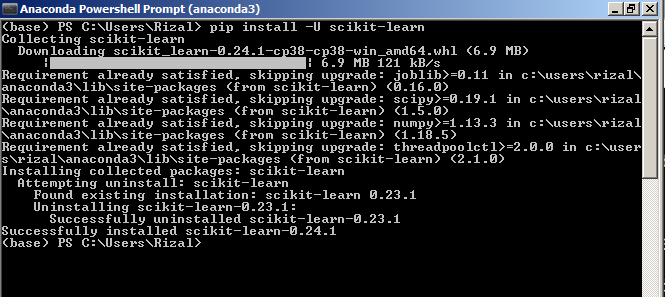
\includegraphics[width=.8\textwidth]{figures/1184033/chapter1/1.PNG}
\end{center}

    

\subsection{Loading an example dataset}
codingan

\begin{center}
    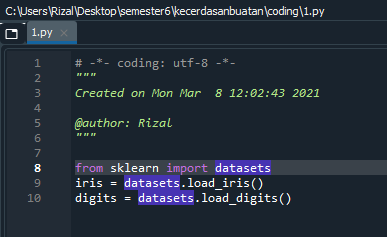
\includegraphics[width=.8\textwidth]{figures/1184033/chapter1/2.PNG}
\end{center}

keterangan
\begin{enumerate}
\item baris 1 mengimport module dataset
\item baris 2 iris ini adalah variable yang digunakan untuk menampung nilai datasets
\item baris 3 digunakan untuk menampung datasets diggit
\end{enumerate}
Hasilnya:
\begin{center}
    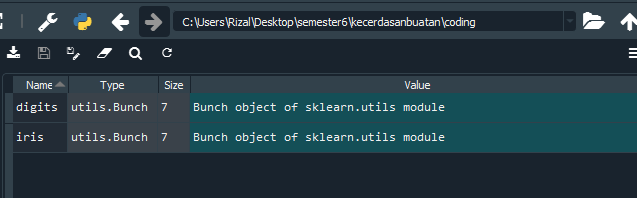
\includegraphics[width=.8\textwidth]{figures/1184033/chapter1/3.PNG}
\end{center}

disini kita akan menampilkan digit data untuk menampilkan seperti dibawah ini
\begin{center}
    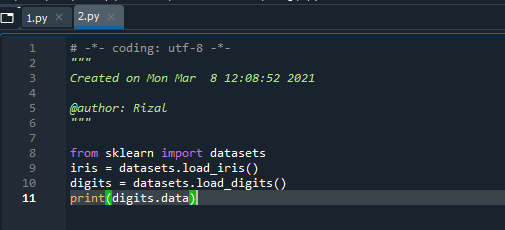
\includegraphics[width=.8\textwidth]{figures/1184033/chapter1/4.PNG}
\end{center}

akan di tambahkan print untuk menampilkan datanya seperti di bawah ini
\begin{center}
    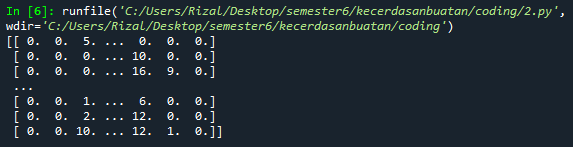
\includegraphics[width=.8\textwidth]{figures/1184033/chapter1/5.PNG}
\end{center}

selain dari digit data kita juga bisa menampilkan target seperti dibawah ini

\begin{center}
    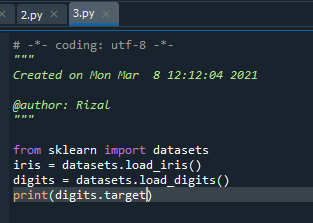
\includegraphics[width=.8\textwidth]{figures/1184033/chapter1/6.PNG}
\end{center}

dan ketika di print hasil nya akan seperti ini

\begin{center}
    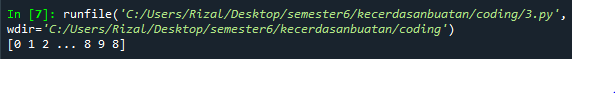
\includegraphics[width=.8\textwidth]{figures/1184033/chapter1/7.PNG}
\end{center}

dan data nya selalu berupa 2D dan setiap sample asli adalah gambar bentuk (8,8),dan cara akses nya bisa dilakukandengan cara berikut ini
\begin{center}
    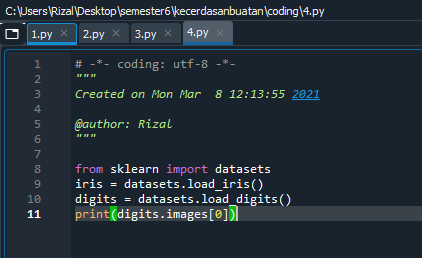
\includegraphics[width=.8\textwidth]{figures/1184033/chapter1/8.PNG}
\end{center}

dan hasilnya akan seperti dibawah ini

\begin{center}
    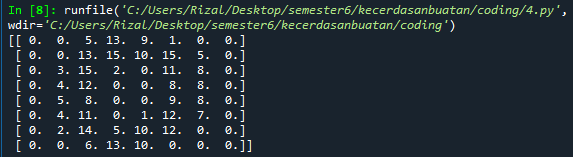
\includegraphics[width=.8\textwidth]{figures/1184033/chapter1/9.PNG}
\end{center}


\subsection{Learning and predicting}

codingan

\begin{center}
    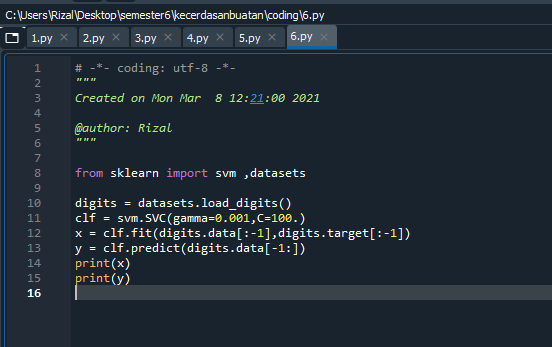
\includegraphics[width=.8\textwidth]{figures/1184033/chapter1/12.PNG}
\end{center}

keterangan
\begin{enumerate}
\item baris 8 mengimport module svm dan datasets dari library sklearn
\item baris 10 iris ini adalah variable yang digunakan untuk menampung nilai datasets
\item baris 11 clf yang memiliki value gamma=0.001 dan Classification = 100diggits digunakan untuk menampung datasets diggitmemiliki nilai untuk memuat dataset digit.
\item baris 12 classifier x
\item baris 13 classifier y
\item baris 14 dan 15 untuk menampilkan nilai
\end{enumerate}
Hasilnya:
\begin{center}
    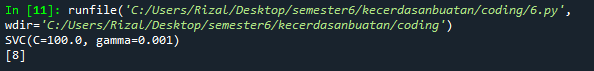
\includegraphics[width=.8\textwidth]{figures/1184033/chapter1/13.PNG}
\end{center}

\subsection{Conventions}
codingan

\begin{center}
    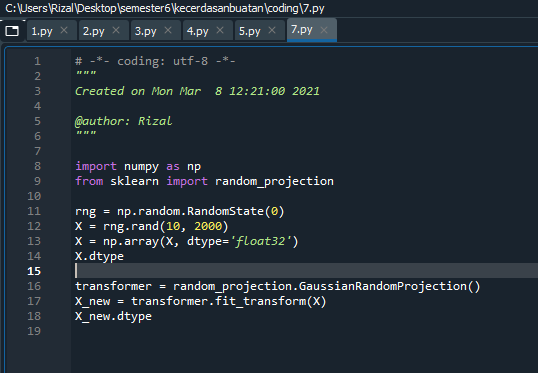
\includegraphics[width=.8\textwidth]{figures/1184033/chapter1/15.PNG}
\end{center}

keterangan
\begin{enumerate}
\item Baris 8 memanggil library numpy dan dibuat dengan alias np.
\item Baris 9 memanggil module random projection dari library sklearn.
\item Baris 11 adalah variable rng yang mendefinisikan numpy as np, kemudian fungsi random dan attr RandomState.
\item Baris 12 adalah variable X yang mendefinisikan variable rng, kemudian method random yang akan menentukan nilai random dari 10 - 2000.
\item Baris 13 adalah variable X yang akan menampung nilai random sebelumnya kedalam array dengan tipe data float32.
\item Baris 14, akan mengubah tipe data nilai random float32 ke float64.
\item Baris 16 adalah sebuah variable transformer yang mendefinisikan class random projection dan memanggil fungsi GaussianRandomProjection.
\item Baris 17 adalah variable X new yang akan melakukan perhitungan pada variable X.
\item Baris 18, merubah tipe data menjadi float64.
\end{enumerate}
Hasilnya:
\begin{center}
    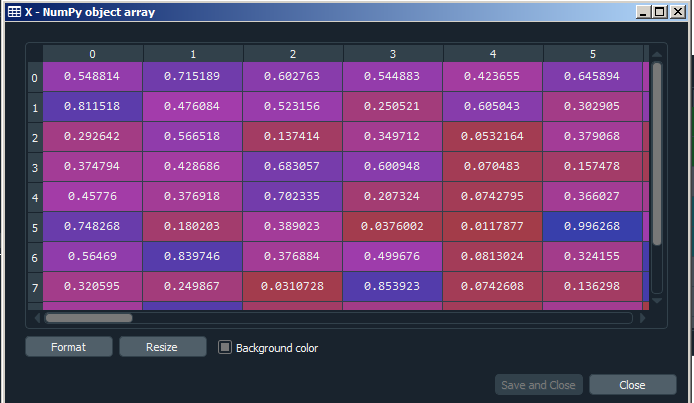
\includegraphics[width=.8\textwidth]{figures/1184033/chapter1/17.PNG}
\end{center}

xnew
\begin{center}
    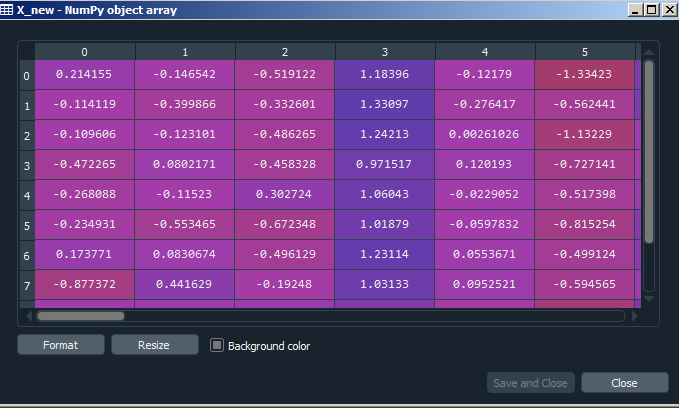
\includegraphics[width=.8\textwidth]{figures/1184033/chapter1/18.PNG}
\end{center}

pad kodingan ini predict () pertama kali mengembalikan array integer, karena iris.target (array integer) digunakan dengan tepat. Prediction () kedua mengembalikan larik string karena iris.target names cocok untuk penginstalan.

\begin{center}
    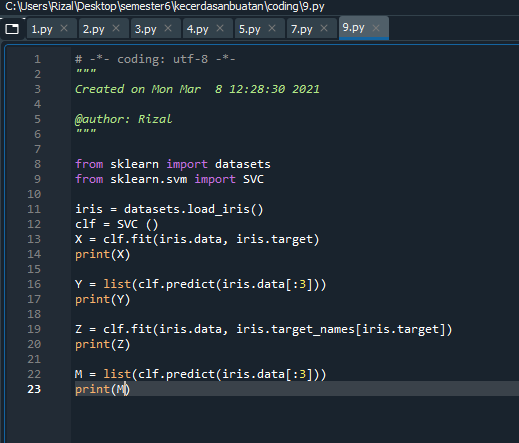
\includegraphics[width=.8\textwidth]{figures/1184033/chapter1/21.PNG}
\end{center}

keterangan
\begin{enumerate}
\item Baris 8, memanggil module datasets dari library sklearn.
\item Baris 9, memanggil module SVC dari library sklearn.svm.
\item Baris 11, variable iris yang memuat datasets iris.
\item Baris 12, variable clf yang memanggil method SVC.
\item Baris 13, variable X yang memanggil classifier kemudian method fit yang memanggil data pas dari iris.data dan target.
\item Baris 14, menampilkan hasil variable X.
\item Baris 15, variable Y yang akan mengembalikan iris predict dalam bentuk array.
\item Baris 16, menampilkan hasil variable Y.
\item Baris 17, memanggil classifier kemudian method fit yang memanggil data pas dari iris.names, iris.data, dan target.
\item Baris 18, menampilkan hasil variable Z.
\item Baris 19, variable M yang akan mengembalikan iris predict kedalam bentuk string.
\item Baris 20, menampilkan hasil variable M.
    \end{enumerate}

Hasil dari iris predict

\begin{center}
    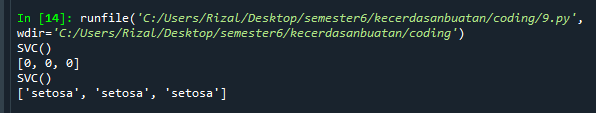
\includegraphics[width=.8\textwidth]{figures/1184033/chapter1/22.PNG}
\end{center}

\subsubsection{Multiclass vs. multilabel fitting}

Coding
    \begin{center}
    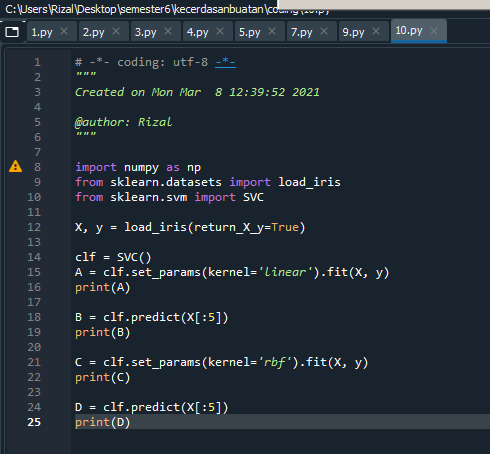
\includegraphics[width=12cm]{figures/1184033/chapter1/23.PNG}
    \end{center}

Keterangan:
    \begin{enumerate}
\item Baris 8, memanggil library numpy dengan alias np.
\item Baris 9, memanggil module load iris dari library sklearn.datasets.
\item Baris 10, memanggil module SVC dari library sklearn.svm.
\item Baris 12, mengisi variable X dan y dengan datasets iris.
\item Baris 14, mendifinisikan clf sebagai fungsi SVC.
\item Baris 15, mengubah rbf menjadi linear melalui SVC.setparams kedalam variable A.
\item Baris 16, menampilkan hasil variable A.
\item Baris 18, clf dengan method predict akan menampilkan data X dalam array sebanyak 5 data kedalam variable B.
\item Baris 19, menampilkan hasil variable B.
\item Baris 21, mengubah linear ke rbf melalui SVC.setparams kedalam variable C.
\item Baris 22, menampilkan hasil variable C.
\item Baris 24, clf dengan method predict akan menampilkan data X dalam array sebanyak 5 data kedalam variable D.
\item Baris 25, menampilkan hasil variable D.
\end{enumerate}

Hasil dari Refitting and updating parameters.
    
    \begin{center}
    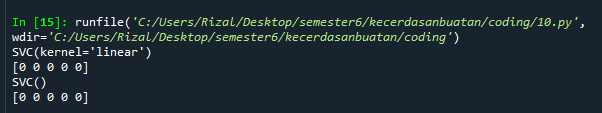
\includegraphics[width=12cm]{figures/1184033/chapter1/24.PNG}
    \end{center}


Di sini, kernel default rbf pertama-tama diubah menjadi linier oleh SVC.setparams () setelah membuat estimator, dan kemudian diubah kembali ke rbf untuk mereparasi estimator dan membuat prediksi kedua.

\subsubsection{Multiclass vs. multilabel fitting}

Saat menggunakan multiclass classifiers, tugas learning and prediction yang dilakukan bergantung pada format data target yang sesuai, yang bergantung pada:

    \begin{center}
    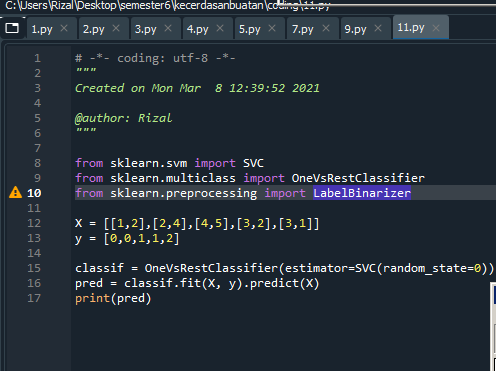
\includegraphics[width=12cm]{figures/1184033/chapter1/25.PNG}
    \end{center}

Keterangan:
    \begin{enumerate}
\item Baris 8, memanggil module SVC dari library sklearn.svm.
\item Baris 9, memanggil module OneVsRestClassifier dari library sklearn.multiclass.
\item Baris 10, memanggil module LabelBinarizer dari library sklearn.preprocessing.
\item Baris 12 dan 13, variable x dan y yang berisi data array.
\item Baris 15, menggunakan method OneVsRestClassifier dengan fungsi SVC sebagai estimator untuk menghasilkan data random yang didefiniskan kedalam classif.
\item Baris 16, memberikan hasil multiclass prediksi yang sesuai kedalam variable pred.
\item Baris 17, menampilkan hasil variable pred.
    \end{enumerate}

Hasil dari Multiclass Predict.
    \begin{center}
    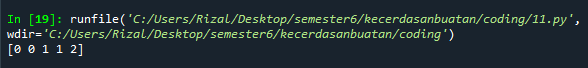
\includegraphics[width=12cm]{figures/1184033/chapter1/26.PNG}
    \end{center}


classifier cocok untuk pred label multiclass, sehingga metode predict () menyediakan prediksi multiclass yang sesuai. Dimungkinkan juga untuk menyesuaikan dengan array 2d indikator label biner:

    \begin{center}
    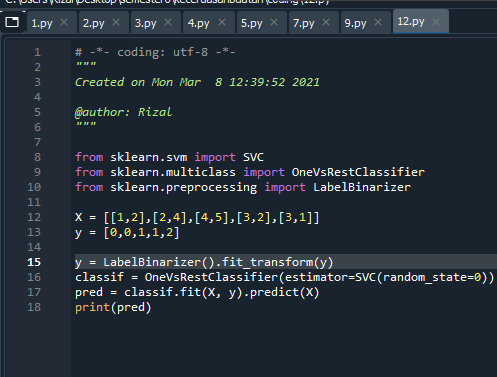
\includegraphics[width=12cm]{figures/1184033/chapter1/27.PNG}
    \end{center}
Keterangan:
    \begin{enumerate}
        \item Baris 8, memanggil module SVC dari library sklearn.svm.
        \item Baris 9, memanggil module OneVsRestClassifier dari library sklearn.multiclass.
        \item Baris 10, memanggil module LabelBinarizer dari library sklearn.preprocessing.
        \item Baris 12 dan 13, variable x dan y yang berisi data array.
        \item Baris 15, classifier fit() merepresentasi variable y dengan LabelBinarizer.
        \item Baris 16, menggunakan method OneVsRestClassifier dengan fungsi SVC sebagai estimator untuk menghasilkan data random yang didefiniskan kedalam classif.
        \item Baris 17, memberikan hasil multiclass prediksi yang sesuai kedalam variable pred.
        \item Baris 18, menampilkan hasil variable pred. 
    \end{enumerate}

Hasil dari Multiclass Predict 2
    
    \begin{center}
    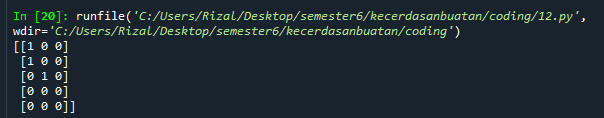
\includegraphics[width=12cm]{figures/1184033/chapter1/28.PNG}
    \end{center}

Di sini, LabelBinarizer digunakan untuk menyesuaikan pengklasifikasi dengan representasi label biner pred dari y. Dalam kasus ini, predict () mengembalikan pred dalam bentuk array yang mewakili prediksi yang sesuai.

MultiLabel Fitting, dalam kasus ini, beberapa label ditetapkan ke classifier yang sesuai untuk setiap sampel. MultiLabelBinarizer digunakan untuk membuat binarisasi pred multilabel agar sesuai. Akibatnya, predict () mengembalikan larik pred yang berisi beberapa label yang diprediksi untuk setiap instance.
    
    \begin{center}
    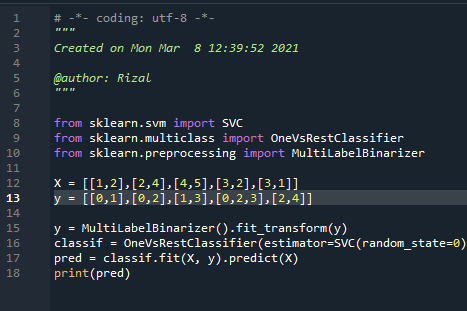
\includegraphics[width=12cm]{figures/1184033/chapter1/29.PNG}
    \end{center}
   
Keterangan:
    \begin{enumerate}
\item Baris 8, memanggil module SVC dari library sklearn.svm.
\item Baris 9, memanggil module OneVsRestClassifier dari library sklearn.multiclass.
\item Baris 10, memanggil module LabelBinarizer dari library sklearn.preprocessing.
\item Baris 12 dan keenam, variable x dan y yang berisi data array.
\item Baris 13, classifier fit() merepresentasi variable y dengan MultiLabelBinarizer.
\item Baris 16, menggunakan method OneVsRestClassifier dengan fungsi SVC sebagai estimator untuk menghasilkan data random yang didefiniskan kedalam classif.
\item Baris 17, memberikan hasil multiclass prediksi yang sesuai kedalam variable pred.
\item Baris 18, menampilkan hasil variable pred. 
    \end{enumerate}

Hasil dari Multilabel Fitting
    \begin{center}
    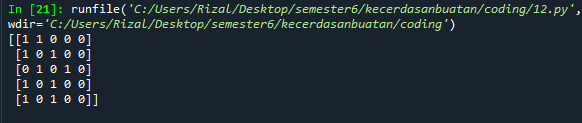
\includegraphics[width=12cm]{figures/1184033/chapter1/30.PNG}
    \end{center}

\section{Error}
Pada saat praktikum, saya mengalami beberapa error, seperti:
\begin{center}
    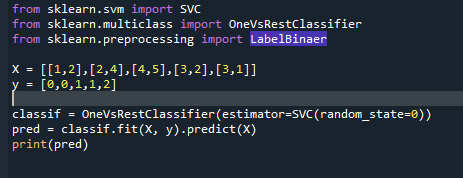
\includegraphics[width=.8\textwidth]{figures/1184033/chapter1/error1.PNG}
\end{center}
gagal mengimport modul karena salah dari penulisan
\begin{center}
    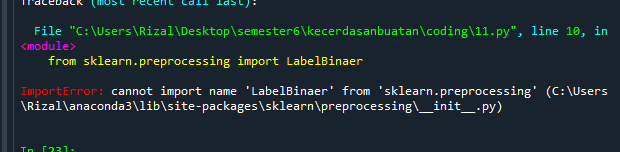
\includegraphics[width=.8\textwidth]{figures/1184033/chapter1/error2.PNG}
\end{center}
Hal ini disebabkan karena adanya kesalahan dalam penulisan kode atau tanda baca.

\begin{center}
    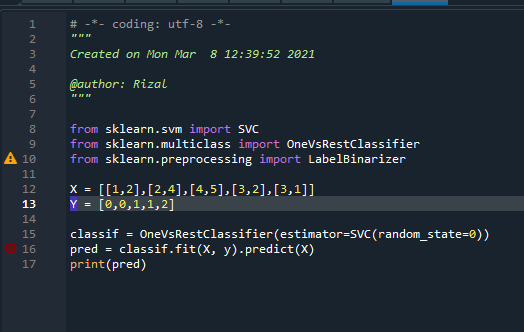
\includegraphics[width=.8\textwidth]{figures/1184033/chapter1/error3.PNG}
\end{center}
gagal menjalankan codingan karenakarena salah dari penulisan
\begin{center}
    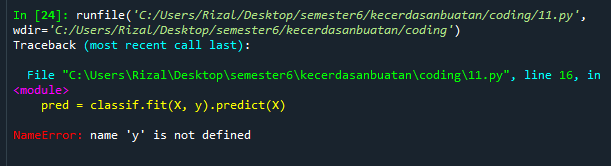
\includegraphics[width=.8\textwidth]{figures/1184033/chapter1/error4.PNG}
\end{center}
Hal ini disebabkan karena adanya kesalahan dalam penulisan kode atau tanda baca jadi harus di perhatikan dalam penulisan.
\end{document}




\end{document}